\documentclass[10pt,a4paper]{amsart}
\usepackage[margin=19mm]{geometry}
\usepackage{amsmath,amssymb,mathtools}
\usepackage[scr=rsfs,cal=euler]{mathalfa}
\usepackage{xfrac}
\usepackage[unicode,hidelinks,bookmarks=false]{hyperref}
\newcommand{\ie}{i.e.\ }
\newcommand{\cf}{cf.\ }
\newcommand{\resp}{respectively\ }
\newcommand{\Subsection}{\subsection}
\providecommand{\nobreakdash}{\nobreak\hbox{-}}
\setlength{\emergencystretch}{2em}
\multlinegap0pt
\usepackage{tikz}
\usepackage{amssymb}
\usepackage{xcolor}
\newtheorem{lemma}{Lemma}
\newcommand{\A}{{\mathfrak a}}
\newcommand{\B}{{\mathfrak b}}
\newcommand{\C}{{\mathfrak c}}
\def\aut{\mathop{\mathrm{Aut}}\nolimits}
\DeclareMathOperator{\cat}{CAT(0)}
\newcommand{\hA}{\hat{\mathfrak a}}
\newcommand{\hB}{\hat{\mathfrak b}}
\newcommand{\hC}{\hat{\mathfrak c}}
\title{On the Girth of Groups Acting on CAT(0) Cube Complexes}
\author{Arka banerjee, Daniel Gulbrandsen, Pratyush Mishra, Prayagdeep Parija}
\date{Source: arXiv:2408.09091v1 (CC BY 4.0)}
\begin{document}
\maketitle

\noindent\emph{Source and licence.} On the Girth of Groups Acting on CAT(0) Cube Complexes. Version arXiv:2408.09091v1 (CC BY 4.0), distributed by arXiv under the Creative Commons Attribution 4.0 International licence, http://creativecommons.org/licenses/by/4.0/, as recorded in the arXiv licence metadata for this exact version and shown on the abstract page https://arxiv.org/abs/2408.09091v1. Full licence notice: \texttt{licenses/arxiv-2408.09091-CC-BY-4.0.txt}.\par\smallskip

\noindent\textit{Editorial scope.} Counted unit: the article's lemma hyperplanes (source0.tex lines 411--413). The article's complete original proof of it is delivered with it (source0.tex lines 421--445, one \texttt{proof} environment of 25 lines, which the article places away from the statement). No mathematics is written, repaired or re-derived: the statement and the proof are the article's own lines, in the article's own notation, and no retained line is substituted or re-flowed.  Retained uncounted as the source-local context the proof needs: lines 447--473.  Nothing was omitted from any retained span, so the package carries no omission record.  No retained line contains a citation, so the wrapper carries no bibliography and no bibliography entry.  The retained lines contain the article's own diagram code, which the wrapper typesets with the standard tikz packages; no image file is delivered and the package declares no asset dependency.  Editorial formatting only, in addition: an AMS \texttt{amsart} preamble that restates the article's own declarations and macros used by the retained lines, namely the environments \texttt{lemma} on separate counters, together with the standard packages those lines need.  The retained environments print in this document as Lemma 1 in order of appearance, whereas the article prints the same items with the numbering of its own full document.  The complete native source of the article as distributed in the arXiv e-print for this exact version is bundled unchanged as \texttt{sources/163883/source0.tex}.
\begin{figure}[htp]\label{f:flipping hyperplanes}
    \centering
    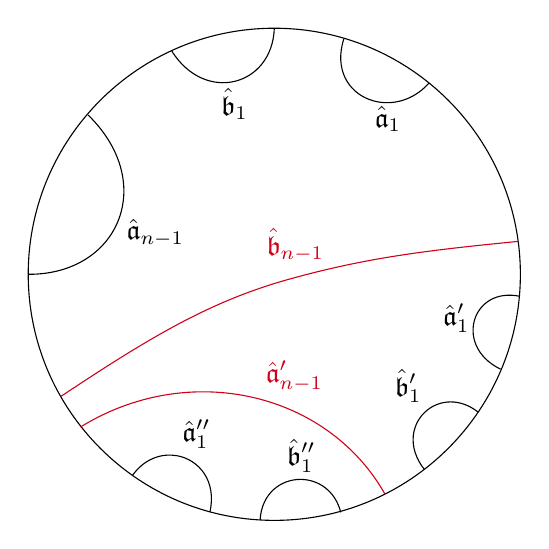
\begin{tikzpicture}[x=0.55pt,y=0.55pt,yscale=-1,xscale=1]

\draw   (169,198.67) .. controls (169,109.38) and (241.38,37) .. (330.67,37) .. controls (419.95,37) and (492.33,109.38) .. (492.33,198.67) .. controls (492.33,287.95) and (419.95,360.33) .. (330.67,360.33) .. controls (241.38,360.33) and (169,287.95) .. (169,198.67) -- cycle ;
\draw [color={rgb, 255:red, 208; green, 2; blue, 27 }  ,draw opacity=1 ]   (190.33,279) .. controls (250.33,239) and (289.45,216.1) .. (340.31,201.92) .. controls (349.56,199.33) and (358.43,197.07) .. (367.11,195.05) .. controls (406.14,185.97) and (441.43,181.91) .. (491.33,177) ;
\draw [color={rgb, 255:red, 208; green, 2; blue, 27 }  ,draw opacity=1 ]   (203.33,299) .. controls (240.83,275.87) and (283.68,270.7) .. (321.4,280.74) .. controls (355.44,289.79) and (385.31,311.22) .. (403.33,343) ;
\draw    (321.33,360) .. controls (322.41,342.26) and (335.33,333.19) .. (348.29,333.41) .. controls (359.45,333.6) and (370.63,340.66) .. (374.33,355) ;
\draw    (237.33,331) .. controls (245.12,319.93) and (256.44,316.09) .. (266.54,317.82) .. controls (281.06,320.31) and (293.05,334.35) .. (288.33,355) ;
\draw    (479.33,261) .. controls (463.03,253.11) and (458.62,238.59) .. (462.61,227.46) .. controls (466.21,217.43) and (476.64,210.16) .. (491.33,213) ;
\draw    (429.33,327) .. controls (417.39,311.8) and (421.07,296) .. (431.09,287.94) .. controls (439.53,281.16) and (452.45,279.86) .. (464.33,289) ;
\draw    (169,198.67) .. controls (201.22,198.85) and (223.61,181.24) .. (229.98,157.9) .. controls (235.34,138.26) and (229.36,114.57) .. (208.33,94) ;
\draw    (263.33,52) .. controls (274.28,69.42) and (290.68,75.19) .. (304.55,71.92) .. controls (318.56,68.62) and (330,56.09) .. (330.67,37) ;
\draw    (376.33,44) .. controls (369.99,64.09) and (379.3,78.59) .. (393.03,83.81) .. controls (405.27,88.45) and (421.02,85.73) .. (432.33,73) ;

\draw (395.03,86.81) node [anchor=north west][inner sep=0.75pt]   [align=left] {$\displaystyle \hat{\mathfrak{a}}_{1}$};
\draw (304.55,74.92) node [anchor=north] [inner sep=0.75pt]   [align=left] {$\displaystyle \hat{\mathfrak{b}}_{1}$};
\draw (231.98,160.9) node [anchor=north west][inner sep=0.75pt]   [align=left] {$\displaystyle \hat{\mathfrak{a}}_{n-1}$};
\draw (365.11,192.05) node [anchor=south east] [inner sep=0.75pt]  [color={rgb, 255:red, 208; green, 2; blue, 27 }  ,opacity=1 ] [align=left] {$\displaystyle \hat{\mathfrak{b}}_{n-1}$};
\draw (323.4,277.74) node [anchor=south west] [inner sep=0.75pt]  [color={rgb, 255:red, 208; green, 2; blue, 27 }  ,opacity=1 ] [align=left] {$\displaystyle \hat{\mathfrak{a}} '_{n-1}$};
\draw (268.54,314.82) node [anchor=south west] [inner sep=0.75pt]   [align=left] {$\displaystyle \hat{\mathfrak{a}} ''_{1}$};
\draw (348.29,330.41) node [anchor=south] [inner sep=0.75pt]   [align=left] {$\displaystyle \hat{\mathfrak{b}} ''_{1}$};
\draw (460.61,227.46) node [anchor=east] [inner sep=0.75pt]   [align=left] {$\displaystyle \hat{\mathfrak{a}} '_{1}$};
\draw (429.09,284.94) node [anchor=south east] [inner sep=0.75pt]   [align=left] {$\displaystyle \hat{\mathfrak{b}} '_{1}$};
\end{tikzpicture}
\caption{The above picture shows how to increase the number of facing hyperplanes. The input is four facing hyperplanes $\{\hA_1,\hB_1,\hA_{n-1},\hB_{n-1}\}$ and the output is six facing hyperplanes $\{\hA_1,\hB_1,\hA'_1,\hB'_1, \hA''_1,\hB''_1\}$.}
\end{figure}

\begin{lemma}[Abundance of facing hyperplanes]\label{l:many facing hyperplanes}
    Let $X$ be an irreducible finite dimensional $\cat$ cube complex where $\aut(X)$ acts essentially and without fixed points at infinity. Let $\{\hA,\hB,\hC\}$ be a facing triple in $X$ with $\hA$ and $\hB$ strongly separated. Then for any $n$, there exists a collection of $2n$ facing hyperplanes $\{\hA_1=\hA,\hB_1=\hB,\hA_2,\hB_2,\ldots,\hA_n,\hB_n\}$ such that each pair $\{\hA_i,\hB_i\}$ is strongly separated for all $i$.
\end{lemma}

\begin{proof}[Proof of Lemma \ref{l:many facing hyperplanes}]
        It is convenient to prove the lemma in terms of the halfspaces.
   Suppose $(\A,\B,\C)$ is the facing triple of halfspaces.
    Let $\A_1:=\A$ and $\B_1:=\B$.
    We start by applying an automorphism to the pair $(\A_1,\B_1)$ that flips the halfspace $\C^*$ to get the pair $(\A_2,\B_2)$.
    Clearly the $\{\A_1,\B_1,\A_2,\B_2\}$ are facing halfspaces and the pair $\{\hA_2,\hB_2\}$ is strongly separated.
    By induction, suppose we have constructed the $2(n-1)$ facing halfspaces $\{\A_1,\B_1,\A_2,\B_2,\ldots,\A_{n-1},\B_{n-1}\}$ such that $\hA_i$ and $\hB_i$ are strongly separated for each $i$ where $n\geq 2$.
    To construct $2n$ facing hyperplanes, we apply an automorphism to the triple  $(\A_1,\B_1,\A_{n-1})$ that flips $\B^*_{n-1}$ to get $(\A'_1,\B'_1,\A'_{n-1})$ 
      and then apply another automorphism to the pair $(\A'_1,\B'_1)$ that flips $\A'^*_{n-1}$ to get another pair $(\A''_1,\B''_1)$ [See figure \ref{f:flipping hyperplanes}].
    By construction, $\{\A'_1,\B'_1\}$ and $\{\A''_1,\B''_1\}$ are both pairs of strongly separated hyperplanes.
    Finally, we claim that the collection $\{\A_1,\B_1,\ldots,\A_{n-2},\B_{n-2},\A'_1,\B'_1,\A''_1,\B''_1\}$ consists of facing halfspaces [Figure \ref{f:flipping hyperplanes}].
    \medskip

    First, we observe that halfspaces in the collection $\{\A_1',\B_1',\A''_2,\B''_2\}$ are mutually disjoint. This is because $\A_1'$ and $\B_1'$ are contained in $\A'^*_{n-1}$, and the pair $(\A''_1,\B''_1)$ is obtained by applying an automorphism to the pair $(\A'_1,\B'_1)$ that flips $\A'^*_{n-1}$. It follows that both $\A''_1$ and $\B''_1$ are contained inside $\A'_{n-1}$. The claim follows.
    \medskip
Next we show that both $\A'_1$ and $\B'_1$ are disjoint from the collection $\{\A_1,\B_1,\ldots,\A_{n-2},\newline \B_{n-2}\}$.
By construction, $(\A'_1,\B'_1)$ is obtained by applying an automorphism to the pair  $(\A_1,\B_1)$ that flips $\B^*_{n-1}$, therefore both $\A'_1$ and $\B'_1$ are  contained inside $\B_{n-1}$.
Since $\B_{n-1}$ is disjoint from any set from the collection $\{\A_1,\B_1,\ldots,\A_{n-2},\B_{n-2}\}$, so are both $\A'_1$ and $\B'_1$.
    \medskip

Similarly, we can show  both $\A''_1$ and $\B''_1$ are disjoint from the collection $\{\A_1,\B_1,\ldots, \newline \A_{n-2},\B_{n-2}\}$.   
    First note that, $\A'_{n-1}\subset \B_{n-1}$ by construction.
    Also, $\A''_1\subset \A'_{n-1}$ and $\B''_1\subset \A'_{n-1}$.
    Consequently both $\A''_1$ and $\B''_1$ are contained inside $\B_{n-1}$ which is disjoint from any set from the collection  $\{\A_1,\B_1,\ldots,\A_{n-2},\B_{n-2}\}$. This finishes the proof.   
   \end{proof}

\end{document}
